\documentclass[12pt,a4paper]{report}

\usepackage[T1]{fontenc}
\usepackage{graphicx}
\usepackage{url}
\usepackage{setspace}
\usepackage{times}
\usepackage{hyperref}
\usepackage[nottoc,notlot,notlof]{tocbibind}
\usepackage{amsmath}
\usepackage{amssymb}
\usepackage{caption}
\usepackage{subcaption}
\usepackage{booktabs}
\usepackage{array}
\usepackage{tikz}
\usepackage{pgfplots}
\pgfplotsset{compat=1.18}
\usetikzlibrary{shapes.geometric, arrows, arrows.meta, positioning, fit, backgrounds, calc}
\usepackage[left=3.5cm,top=2cm,right=3cm,bottom=4cm]{geometry}
\setcounter{tocdepth}{2}
\usepackage{listings}
\usepackage{xcolor}

\renewcommand{\baselinestretch}{1.25}
\renewcommand{\bibname}{References}
\renewcommand\listfigurename{\centering{List of Figures}}
\renewcommand\listtablename{\centering{List of Tables}}

%% ---- Code listing style ----
\lstset{
  basicstyle=\ttfamily\small,
  keywordstyle=\color{blue}\bfseries,
  commentstyle=\color{gray},
  stringstyle=\color{red!70!black},
  backgroundcolor=\color{gray!5},
  frame=single,
  framerule=0.4pt,
  breaklines=true,
  columns=fullflexible,
  showstringspaces=false,
  tabsize=4,
  captionpos=b,
}

%% ---- TikZ styles ----
\tikzstyle{process}   = [rectangle, rounded corners, minimum width=3.2cm, minimum height=1cm,
                          text centered, draw=black, fill=blue!15, text width=3cm]
\tikzstyle{entity}    = [rectangle, minimum width=2.8cm, minimum height=1cm,
                          text centered, draw=black, fill=orange!20, text width=2.6cm]
\tikzstyle{datastore} = [rectangle, minimum width=3cm, minimum height=0.8cm,
                          text centered, draw=black, fill=yellow!25,
                          double, double distance=2pt, text width=3cm]
\tikzstyle{arrow}     = [thick,->,>=stealth]
\tikzstyle{darrow}    = [thick,<->,>=stealth]

\begin{document}

%% ============================================================
%%  TITLE PAGE
%% ============================================================
\begin{titlepage}
\begin{center}
{\LARGE \textbf{Hybrid Knowledge-Graph-Enhanced\\[0.2cm]
Retrieval-Augmented Generation for\\[0.2cm]
Academic Information Systems}}\\[0.2cm]
\vspace{1cm}
{\Large \textbf{A Mini Project Report}}\\
\vspace{0.4cm}
\large \textit{Submitted to the APJ Abdul Kalam Technological University}\\
\vspace{0.1cm}
\large \textit{in partial fulfillment of requirements for the award of degree}\\
\vspace{0.8cm}
{\Large \textbf{Bachelor of Technology}}\\
\vspace*{0.1cm}
\large{in}\\
\vspace*{0.1cm}
{\Large \textbf{Computer Science and Engineering}}\\
\vspace*{0.1cm}
\large \em{by}\\
\vspace*{0.1cm}
{\Large \textbf{\scshape{Julia Mariam John}}}\,({\textbf{B23CS2137}})\\
{\Large \textbf{\scshape{Nirmel B Joseph}}}\,({\textbf{B23CS2148}})\\
{\Large \textbf{\scshape{Rohith NS}}}\,({\textbf{B23CS2156}})\\
\vspace*{1cm}
\centerline{
\includegraphics[width=5cm]{logo.png}}
\vspace*{-1cm}
\begin{center}
  {\bf \large Department of Computer Science and Engineering}\\
  {\bf \large Mar Baselios College of Engineering and Technology (Autonomous)}\\
  {\bf \large Mar Ivanios Vidya Nagar, Nalanchira}\\
  {\bf \large Thiruvananthapuram--695015}\par
  \vspace{0.3cm}
  {\bf \large April 2026}\\\par
\end{center}
\vfill
\end{center}
\end{titlepage}
\pagebreak
\pagenumbering{gobble}

%% ============================================================
%%  CERTIFICATE
%% ============================================================
\begin{center}
  \textbf{DEPARTMENT OF COMPUTER SCIENCE AND ENGINEERING}\\
  \textbf{MAR BASELIOS COLLEGE OF ENGINEERING AND TECHNOLOGY (AUTONOMOUS)}\\
  \textbf{MAR IVANIOS VIDYA NAGAR, NALANCHIRA}\\
  \textbf{THIRUVANANTHAPURAM--695015}
\end{center}
\begin{center}
  \centerline{
\includegraphics[width=5.5cm]{logo.png}}
\end{center}
\begin{center}
  {\Large \textbf{\scshape{Certificate}}}
\end{center}
\vspace*{.1in}
\setstretch{1.5}
\par
This is to certify that the report entitled \textbf{Hybrid Knowledge-Graph-Enhanced Retrieval-Augmented Generation for Academic Information Systems} submitted by \textbf{Julia Mariam John}~(B23CS2137), \textbf{Nirmel B Joseph}~(B23CS2148) \& \textbf{Rohith NS}~(B23CS2156), to the APJ Abdul Kalam Technological University in partial fulfillment of the B.Tech.\ degree in Computer Science and Engineering is a bonafide record of the mini project work carried out by them under our guidance and supervision. This report in any form has not been submitted to any other University or Institute for any purpose.
\vspace{0.5in}
\begin{singlespacing}
\hspace*{-0.25in}
\parbox{3in}{
  \noindent \textbf{Mr. Praveen J.S} \\
  \noindent (Mini Project Guide) \\
  \noindent Assistant Professor\\
  \noindent Department of CSE\\
}
\hspace*{1in}
\parbox{2.5in}{
  \noindent \textbf{Dr. Merlin George} \\
  \noindent (Mini Project Co-ordinator)\\
  \noindent Assistant Professor\\
  \noindent Department of CSE\\
}\\
\end{singlespacing}
\begin{singlespacing}
\hspace*{2in}
\parbox{2.5in}{
  \noindent \textbf{Dr. Jisha John} \\
  \noindent (Head of the Department)\\
  \noindent Professor\\
  \noindent Department of CSE\\
}
\end{singlespacing}
\begin{singlespacing}
\vspace{0.2in}
\hspace*{-0.25in}
\parbox{2.5in}{\noindent Place: Thiruvananthapuram\\}
\hspace*{1.5in}
\parbox{2.5in}{\noindent Date:\\}
\end{singlespacing}
\clearpage

%% ============================================================
%%  ACKNOWLEDGEMENT
%% ============================================================
\pagenumbering{roman}
\addcontentsline{toc}{chapter}{Acknowledgement}
\begin{center}
  {\Large \textbf{Acknowledgement}}\\[0.5cm]
\end{center}
\vspace*{0.5in}

We express our deepest gratitude to our Mini Project Guide \textbf{Mr. Praveen J.S}, Assistant Professor, Department of Computer Science and Engineering, for providing continuous guidance, critical feedback, and technical insights throughout the development of this project. His expertise in natural language processing and information retrieval systems greatly shaped the direction and quality of this work.

\par
We sincerely thank \textbf{Dr. Merlin George}, Mini Project Co-ordinator, and \textbf{Dr. Jisha John}, Head of the Department of CSE, for their academic support, resource provisioning, and encouragement at every stage of this project.

\par
We acknowledge the open-source communities behind \textbf{ChromaDB}, \textbf{Sentence-Transformers}, \textbf{BeautifulSoup}, \textbf{pdfplumber}, and \textbf{LangChain} — without their tools, building this system would not have been feasible within the project timeframe. We also thank the broader NLP and knowledge graph research communities whose published work on retrieval-augmented generation and graph-enhanced reasoning informed our system design.

\par
Finally, we are grateful to our families and friends for their patience and encouragement throughout this endeavour.

\begin{flushright}
\textbf{\noindent Julia Mariam John}\\
\textbf{\noindent Nirmel B Joseph}\\
\textbf{\noindent Rohith NS}
\end{flushright}
\cleardoublepage

%% ============================================================
%%  ABSTRACT
%% ============================================================
\addcontentsline{toc}{chapter}{Abstract}
\begin{center}
  {\Large \textbf{Abstract}}\\[0.5cm]
\end{center}
\setstretch{1.5}

Academic information hosted on college websites is largely unstructured, heterogeneous, and distributed across multiple webpages, making precise information retrieval difficult using traditional keyword-based search techniques. While retrieval-augmented generation (RAG) has shown effectiveness in grounding large language model outputs using semantic vector retrieval, purely embedding-based approaches often fail to capture explicit relationships among entities such as departments, courses, and faculty, leading to incomplete or contextually weak responses.

\par
This mini project proposes a \textbf{hybrid knowledge-graph-enhanced retrieval-augmented generation framework} for academic information access. Unstructured institutional content from the MBCET CSE department website is processed through web scraping, text cleaning, semantic chunking, and vector embedding, then indexed in a ChromaDB vector database to support similarity-based retrieval. In parallel, a lightweight knowledge graph is constructed to explicitly represent structured academic entities — faculty, courses, programs, and semesters — and their relationships such as \textit{teaches}, \textit{part\_of}, and \textit{has\_prerequisite}.

\par
An intent-aware retrieval mechanism dynamically selects semantic retrieval, graph-based reasoning, or a hybrid of both to construct context for generation. The retrieved evidence is supplied to a large language model to generate grounded responses constrained to institutional knowledge. The data pipeline processes 60+ HTML pages and 10 PDF documents, producing 640 semantic chunks and a validated knowledge graph with deterministic, evidence-backed edges.

\par
This design is motivated by recent journal studies demonstrating that integrating knowledge graphs into RAG pipelines improves factual grounding, relational reasoning, and interpretability, while domain-specific RAG systems enhance retrieval reliability in academic settings~\cite{kg_rag_springer,rag_edu_elsevier}.

\par
\noindent\textbf{Keywords:} Retrieval-Augmented Generation, Knowledge Graph Integration, Vector Embeddings, Semantic Chunking, ChromaDB, Academic Information Systems.

\par
\noindent\textbf{Sustainable Development Goals (SDGs):} This mini project supports SDG~4 (Quality Education) by improving structured access to academic information and SDG~9 (Industry, Innovation and Infrastructure) through the application of hybrid intelligent information retrieval systems.

\clearpage

%% ============================================================
%%  FRONT MATTER
%% ============================================================
\begin{singlespacing}
\hypersetup{linkcolor=black}
\renewcommand\contentsname{\centering{Table of Contents}}
\tableofcontents
\setcounter{secnumdepth}{3}
\clearpage
\addcontentsline{toc}{chapter}{\listfigurename}
\addtocontents{lof}{\hspace{.6cm}\textbf{No.}~\hfill\textbf{Title}~\hfill\textbf{Page No.}\par}
\listoffigures
\clearpage
\addcontentsline{toc}{chapter}{\listtablename}
\addtocontents{lot}{\hspace{.6cm}\textbf{No.}~\hfill\textbf{Title}~\hfill\textbf{Page No.}\par}
\listoftables
\cleardoublepage
\end{singlespacing}

%% ============================================================
%%  CHAPTER 1 — INTRODUCTION
%% ============================================================
\setcounter{page}{1}
\pagenumbering{arabic}
\chapter{Introduction}

The rapid digitisation of higher education has made institutional websites the primary interface between colleges and their stakeholders — students, parents, faculty, and prospective applicants. Yet the information hosted on these websites is typically unstructured, heterogeneous, and distributed across dozens of independently maintained pages. Course syllabi exist as downloadable PDFs, faculty profiles are scattered across departmental sub-pages, examination schedules are buried under nested navigation menus, and academic regulations span multiple revision documents. This fragmentation makes even basic information retrieval a time-consuming and frustrating exercise.

\par
Traditional search engines and site-specific keyword search tools offer little relief. They rely on lexical matching, which fails when a user's natural-language query does not use the exact terminology present in the source document. A student searching for ``who teaches Artificial Intelligence'' will not find the answer if the assignment is listed under a course code in a timetable PDF. The semantic gap between user intent and document surface form is a well-recognised challenge in information retrieval~\cite{kg_rag_springer}.

\par
Retrieval-Augmented Generation (RAG) addresses part of this problem by combining semantic vector retrieval with the generative power of large language models (LLMs). In a RAG pipeline, user queries are embedded into the same vector space as pre-processed document chunks, the most relevant chunks are retrieved via similarity search, and the retrieved context is supplied to an LLM to synthesise a grounded response. This approach dramatically reduces hallucination compared to using an LLM alone, and has shown promising results in educational applications~\cite{rag_edu_elsevier}.

\par
However, purely embedding-based RAG systems exhibit a critical weakness: they treat documents as isolated text passages and fail to capture the \textit{structural relationships} that exist between academic entities. A university's information space is inherently relational — courses belong to programs, faculty teach specific courses, prerequisites link modules across semesters, and departments houses laboratories. These relationships are not merely implied; they are essential for answering multi-hop queries such as ``Which professors in CSE teach semester 5 courses?'' or ``What are the prerequisites for the elective on Machine Learning?''

\par
Knowledge graphs (KGs) offer a natural representation for such structured relationships. By explicitly encoding entities and their typed relationships as nodes and edges, a knowledge graph enables graph-based reasoning that complements the semantic similarity search of vector retrieval. Recent research has demonstrated that integrating knowledge graphs into RAG pipelines significantly improves multi-hop question answering accuracy, factual grounding, and interpretability~\cite{kg_rag_springer}.

\par
This mini project proposes a \textbf{hybrid knowledge-graph-enhanced retrieval-augmented generation system} specifically designed for academic information access. The system targets the Computer Science and Engineering (CSE) department of Mar Baselios College of Engineering and Technology (MBCET), processing its website content through a comprehensive pipeline that includes web scraping, PDF extraction, semantic chunking, vector embedding, knowledge graph construction, and intent-aware hybrid retrieval.

\clearpage

\section{Problem Statement}

To develop a hybrid knowledge-graph-enhanced retrieval-augmented generation system that provides accurate, contextually grounded, and relationally aware responses to academic information queries using institutional web content.

\par
Specifically, the system must: (a)~scrape and process unstructured content from the MBCET CSE department website, including HTML pages and PDF syllabi; (b)~construct semantic vector embeddings and store them in a vector database for similarity-based retrieval; (c)~build a lightweight knowledge graph that explicitly represents academic entities (faculty, courses, programs) and their relationships (teaches, part\_of, has\_prerequisite); (d)~implement an intent-aware query router that dynamically selects semantic retrieval, graph-based retrieval, or a hybrid of both; and (e)~generate grounded, natural-language responses using a large language model constrained to retrieved institutional knowledge.

\section{Objectives}

\begin{enumerate}
  \item To collect academic data from institutional websites using automated web scraping techniques.
  \item To convert the collected text data into vector embeddings using semantic embedding models for similarity-based retrieval.
  \item To construct a knowledge graph of academic entities for Mar Baselios College of Engineering and Technology.
  \item To integrate hybrid retrieval combining vector similarity search and knowledge graph reasoning for query answering.
  \item To improve factual grounding and relational reasoning in LLM-generated responses for academic queries.
\end{enumerate}

\section{Scope}

The system targets the MBCET CSE department website (\texttt{mbcet.ac.in/cse}) as its primary data source. The data pipeline processes approximately 60 HTML pages and 10 PDF documents (syllabi, regulations, and academic calendars). The semantic chunker generates approximately 640 text chunks, each classified by content type (profile, regulation, table, section, list). The knowledge graph captures faculty, course, program, and semester entities with deterministic, evidence-backed edges. The system is designed for deployment on standard development hardware (Python 3.11, no GPU required for inference) and does not require proprietary APIs for its core retrieval pipeline.
\clearpage

%% ============================================================
%%  CHAPTER 2 — LITERATURE REVIEW
%% ============================================================
\chapter{Literature Review}

The intersection of retrieval-augmented generation and knowledge graph reasoning has attracted significant research attention in recent years, driven by the need to improve the factual accuracy and relational reasoning capabilities of large language model systems. This chapter reviews the key works that inform the design of the proposed hybrid KG-RAG system.

\section{Retrieval-Augmented Generation}

Lewis~\textit{et al.}~\cite{lewis2020} introduced RAG as a general-purpose fine-tuning method for knowledge-intensive NLP tasks. Their architecture combines a pre-trained parametric memory (BART generator) with a non-parametric memory (Dense Passage Retriever + Wikipedia index), allowing the model to access and condition on retrieved documents during generation. This foundational work established that retrieval augmentation significantly reduces hallucination and improves factual accuracy compared to closed-book language models.

\par
Subsequent work by Izacard and Grave~\cite{izacard2021} introduced Fusion-in-Decoder (FiD), which encodes each retrieved passage independently before fusing them in the decoder. This approach scales more efficiently to larger numbers of retrieved documents and demonstrated state-of-the-art performance on open-domain QA benchmarks. The core insight — that independently encoding documents preserves passage-level information better than concatenation — informs the chunking strategy adopted in our system.

\section{Knowledge Graphs in NLP}

Knowledge graphs have become an essential component in NLP pipelines for representing structured world knowledge. Hogan~\textit{et al.}~\cite{hogan2021} provide a comprehensive survey of knowledge graph types, construction methods, and applications. In the context of question answering, knowledge graphs enable multi-hop reasoning by following explicit typed relationships between entities — a capability that purely embedding-based retrieval lacks.

\par
Pan~\textit{et al.}~\cite{pan2024} surveyed the unification of large language models and knowledge graphs, identifying three paradigms: (i)~KG-enhanced LLMs, where graph structure guides retrieval or reasoning; (ii)~LLM-enhanced KGs, where language models assist in graph construction and completion; and (iii)~synergised approaches where both systems co-evolve. The proposed system falls under the first paradigm, using a pre-constructed knowledge graph to complement vector retrieval.

\section{Knowledge-Graph-Enhanced RAG}

Linders and Tomczak~\cite{kg_rag_springer} proposed a knowledge-graph-extended RAG framework for question answering. Their approach augments the standard RAG retrieval step with graph-guided retrieval, where the knowledge graph identifies entity relationships that help the retriever surface relevant passages for multi-hop questions. Their experiments showed improved accuracy on complex compositional queries where standard retrieval fails due to the need to combine information from multiple documents.

\par
Li~\textit{et al.}~\cite{rag_edu_elsevier} conducted a systematic survey of RAG applications in educational settings. They found that domain-specific RAG systems, when properly grounded in curated institutional knowledge bases, significantly outperform general-purpose LLMs on tasks requiring factual precision about specific universities, courses, or policies. The survey also identified the lack of structured relational knowledge as a key limitation of existing educational RAG systems — a gap that the proposed hybrid approach directly addresses.

\section{Summary of Related Works}

\begin{table}[h!]
  \centering
  \caption{Summary of Related Works}
  \label{tab:litreview}
  \vspace*{5pt}
  \begin{tabular}{|p{3cm}|p{3.2cm}|p{3cm}|p{3cm}|}
    \hline
    \textbf{Author(s)} & \textbf{Method} & \textbf{Focus} & \textbf{Limitation} \\ \hline
    Lewis et al.\ (2020)    & RAG (DPR + BART)          & Open-domain QA                  & No relational reasoning           \\ \hline
    Izacard \& Grave (2021) & Fusion-in-Decoder         & Multi-document QA               & Scalability to large KBs          \\ \hline
    Linders \& Tomczak (2025)& KG-extended RAG           & Multi-hop QA                    & Requires pre-built KG              \\ \hline
    Li et al.\ (2025)       & RAG survey (education)    & Educational QA                  & Dependent on retriever quality    \\ \hline
    Pan et al.\ (2024)      & LLM-KG unification survey & Knowledge representation        & Broad survey, no implementation   \\ \hline
    \textbf{Proposed System}& Hybrid KG-RAG             & Academic info. retrieval (MBCET) & Limited to single institution  \\ \hline
  \end{tabular}
\end{table}

\section{Gaps in the Literature}

\begin{itemize}
  \item Limited use of knowledge graphs specifically in academic RAG systems for institutional information access.
  \item Lack of hybrid vector-graph retrieval pipelines that dynamically route queries based on intent classification.
  \item Insufficient explainability in LLM-based academic question answering — most systems provide answers without citing structured evidence provenance.
  \item Few open-source, end-to-end implementations that combine web scraping, semantic chunking, knowledge graph construction, and retrieval-augmented generation in a single pipeline.
\end{itemize}

\par
The proposed system directly addresses all four gaps by combining semantic vector retrieval (ChromaDB), a phase-1 deterministic knowledge graph (JSON-based), intent-aware query routing, and evidence-backed answer generation within an open-source, reproducible pipeline.
\clearpage

%% ============================================================
%%  CHAPTER 3 — PROPOSED METHODOLOGY
%% ============================================================
\chapter{Proposed Methodology}

\section{Problem Statement}

Academic information hosted on college websites is largely unstructured, heterogeneous, and distributed across multiple webpages. Traditional keyword-based search techniques fail when users express queries in natural language that does not match the exact terminology in source documents. While retrieval-augmented generation has shown effectiveness in grounding LLM outputs, purely embedding-based approaches fail to capture explicit relationships among entities such as departments, courses, and faculty, leading to incomplete or contextually weak responses.

\par
The core problem addressed in this project is: \textit{Given a user's natural-language query about academic information, how can the system accurately retrieve and synthesise an answer by combining semantic similarity search over document chunks with structured relational reasoning over a knowledge graph of academic entities?}

\par
Specifically, the system must: (a)~ingest unstructured web content (HTML pages and PDF documents) and transform it into semantically meaningful, retrievable chunks; (b)~construct a lightweight knowledge graph capturing relationships between faculty, courses, programs, and semesters; (c)~route incoming queries to the optimal retrieval strategy (vector, graph, or hybrid) based on intent classification; and (d)~generate grounded, natural-language responses constrained to retrieved institutional knowledge.

\subsection*{Objectives}

\begin{itemize}
  \item To collect academic data from the MBCET CSE department website using automated web scraping with BFS URL discovery, HTML-to-Markdown conversion, and PDF table extraction.
  \item To design and implement a semantic chunking pipeline that classifies content by type (profile, regulation, table, section, list) and preserves structural metadata.
  \item To generate vector embeddings using EmbeddingGemma (768-dimensional) and store them in ChromaDB for fast similarity-based retrieval.
  \item To construct a phase-1 knowledge graph with deterministic edges (teaches, part\_of, has\_prerequisite) backed by chunk-level evidence provenance.
  \item To implement an intent-aware query router that classifies queries into types (teaching, faculty, course, regulation, general) and routes them to the optimal retrieval path.
  \item To integrate the retrieved context with a large language model for grounded answer generation.
\end{itemize}

\subsection*{Scope}

The system targets the MBCET CSE department website (\texttt{mbcet.ac.in}) as its primary data source. The data pipeline processes 60+ HTML pages and 10 PDF documents, producing 640 semantic chunks across five content types. The knowledge graph captures faculty (43 entities), courses, programs (B.Tech CSE, B.Tech AI, M.Tech CSE), and semester entities with deterministic, high-confidence edges only. The embedding model (EmbeddingGemma, 768 dimensions) is optimised for a GTX 1650 Ti GPU (4~GB VRAM) with batch size 64 and max sequence length 512 tokens. The system can also run on CPU for inference.

\section{Proposed Methodology}

The proposed system follows a multi-stage pipeline architecture comprising six functional components: data collection, data pre-processing, vector embedding and storage, knowledge graph construction, hybrid retrieval, and answer generation. The novelty of this approach lies in three aspects: (i)~a content-aware semantic chunker that preserves structural metadata and entity references for each chunk, (ii)~a deterministic knowledge graph builder that produces only evidence-backed, high-confidence edges with full provenance tracking, and (iii)~an intent-aware query router with adaptive distance thresholding that dynamically selects the optimal retrieval strategy.

\subsection{Data Collection}

Academic data is collected from the MBCET CSE department website using a BFS-based URL discovery engine implemented in Python. The crawler uses the \texttt{requests} library with configurable delays (1.0s between requests), retry logic (3 retries), and polite user-agent identification. The system discovers and processes two types of content:

\begin{itemize}
  \item \textbf{HTML Pages:} Department overview, faculty profiles, laboratory details, program descriptions, and event listings. These are converted to clean Markdown using \texttt{markdownify} with HTML tag stripping and whitespace normalisation.
  \item \textbf{PDF Documents:} Syllabi (B.Tech CSE, B.Tech AI, M.Tech CSE), academic regulations (R2019, R2023), examination schedules, and academic calendars. PDFs are processed using \texttt{pdfplumber} for text and table extraction, with OCR fallback via Tesseract for scanned documents.
\end{itemize}

\subsection{Semantic Chunking}

The semantic chunker transforms raw Markdown content into structured, retrievable chunks. Unlike naive fixed-size splitting, the chunker is content-aware:

\begin{itemize}
  \item Parses Markdown structure (headers, lists, tables, paragraphs) to identify natural semantic boundaries.
  \item Classifies each chunk into one of five content types: \textbf{profile} (faculty), \textbf{regulation}, \textbf{table} (course lists, timetables), \textbf{section} (general content), and \textbf{list}.
  \item Links chunks to entity references (e.g., faculty IDs, course codes, semester identifiers) for downstream knowledge graph integration.
  \item Enforces configurable chunk size constraints: minimum 80 words, preferred 450 words, soft limit 600 words, maximum 700 words.
  \item Performs SHA-256 based deduplication to eliminate redundant content.
\end{itemize}

\begin{table}[h!]
  \centering
  \caption{Semantic Chunk Schema}
  \label{tab:chunk_schema}
  \vspace*{5pt}
  \begin{tabular}{|l|l|p{6cm}|}
    \hline
    \textbf{Field} & \textbf{Type} & \textbf{Description} \\ \hline
    \texttt{chunk\_id}           & string   & Unique identifier (source + hash)          \\ \hline
    \texttt{text}                & string   & Chunk content in Markdown format           \\ \hline
    \texttt{source\_type}        & string   & ``page'' or ``pdf''                        \\ \hline
    \texttt{source\_file}        & string   & Path to source Markdown file               \\ \hline
    \texttt{section\_hierarchy}  & list     & Nesting of parent headings                 \\ \hline
    \texttt{content\_type}       & string   & profile, regulation, table, section, list  \\ \hline
    \texttt{entity\_refs}        & list     & Linked entity IDs (faculty, course, etc.)  \\ \hline
    \texttt{page\_range}         & list     & Start and end PDF page (if applicable)     \\ \hline
    \texttt{word\_count}         & int      & Number of words in chunk                   \\ \hline
    \texttt{hash}                & string   & SHA-256 content hash for deduplication     \\ \hline
  \end{tabular}
\end{table}

\subsection{Vector Embedding and Storage}

Each semantic chunk is converted into a 768-dimensional vector embedding using the \textbf{EmbeddingGemma} model (\texttt{google/embeddinggemma-300m}) from the Sentence-Transformers library. The embeddings are L2-normalised for cosine similarity and stored in a \textbf{ChromaDB} persistent vector database.

\par
Key implementation details:
\begin{itemize}
  \item Batch size of 64, optimised for 4~GB GPU VRAM (GTX 1650 Ti).
  \item Max sequence length truncated to 512 tokens for performance (default is 2048, which causes approximately 30$\times$ slowdown for long table chunks).
  \item Automatic GPU fallback: on CUDA out-of-memory errors, the batch size is recursively halved; if batch size 1 still fails, the pipeline falls back to CPU.
  \item Embedding cache saved as compressed \texttt{.npz} file for fast re-loading without re-encoding.
  \item Structured metadata (content type, source file, entity references, section hierarchy) stored alongside each vector in ChromaDB for filtered retrieval.
\end{itemize}

\subsection{Knowledge Graph Construction}

A lightweight knowledge graph is constructed from the entity registries and semantic chunks. The phase-1 implementation enforces strict constraints:

\begin{itemize}
  \item \textbf{Storage format:} JSON only (no graph database dependency).
  \item \textbf{Edge policy:} Deterministic, high-confidence edges only (confidence = 1.0).
  \item \textbf{Evidence provenance:} Every edge includes references to the source chunk ID, source file, and extraction rule.
\end{itemize}

\par
The graph contains four node types and three edge types:

\begin{table}[h!]
  \centering
  \caption{Knowledge Graph Node and Edge Types}
  \label{tab:kg_types}
  \vspace*{5pt}
  \begin{tabular}{|l|l|p{6cm}|}
    \hline
    \textbf{Element} & \textbf{Type} & \textbf{Description} \\ \hline
    Node & Faculty   & 43 faculty members with name, aliases, URL     \\ \hline
    Node & Course    & Course code, name, credits, aliases             \\ \hline
    Node & Program   & B.Tech CSE, B.Tech AI, M.Tech CSE               \\ \hline
    Node & Semester  & Semesters 1--8 (deterministic from chunk refs)   \\ \hline
    Edge & teaches          & Faculty $\rightarrow$ Course (from timetable tables) \\ \hline
    Edge & part\_of          & Course $\rightarrow$ Program (from syllabus source)   \\ \hline
    Edge & has\_prerequisite & Course $\rightarrow$ Course (from prerequisite text)   \\ \hline
  \end{tabular}
\end{table}

The edge extraction pipeline uses three rule-based extractors:
\begin{enumerate}
  \item \textbf{Course-Program mapping:} Extracts \texttt{part\_of} edges by matching course entity references in chunks to program identifiers, using both explicit entity co-occurrence and source-file heuristics (e.g., files containing ``cse\_ai'' map to B.Tech AI).
  \item \textbf{Prerequisite extraction:} Uses regex patterns to find \texttt{prerequisite:} annotations in chunk text and maps course codes to course entity IDs.
  \item \textbf{Teaching assignment extraction:} Detects co-occurrence of faculty aliases and course aliases in table rows (signalled by pipe characters) or lines containing assignment cue words (``teaches'', ``handled by'', ``instructor'').
\end{enumerate}

The graph is validated post-construction: every edge must have both endpoints in the node set, confidence must be 1.0, the deterministic flag must be true, and evidence must be non-empty.

\subsection{Hybrid Retrieval}

When a user submits a query, the system performs intent-aware routing:

\begin{enumerate}
  \item \textbf{Query classification:} The query is classified into one of six types: \textit{teaching}, \textit{faculty}, \textit{course}, \textit{timetable}, \textit{regulation}, or \textit{general}.
  \item \textbf{Retrieval routing:} Based on the classified type, the system applies content-type filters in ChromaDB and adjusts the number of results:
    \begin{itemize}
      \item \textit{teaching} $\rightarrow$ filter \texttt{knowledge\_graph} chunks, $k=5$
      \item \textit{faculty} $\rightarrow$ filter \texttt{profile} chunks, $k=3$
      \item \textit{course} $\rightarrow$ filter \texttt{table} chunks, $k=10$
      \item \textit{regulation} $\rightarrow$ filter \texttt{regulation} chunks, $k=5$
      \item \textit{general} $\rightarrow$ no filter, $k=5$
    \end{itemize}
  \item \textbf{Adaptive distance thresholding:} Retrieved results are filtered based on best-match quality:
    \begin{itemize}
      \item Best distance $< 0.3$ (excellent): threshold = 0.6
      \item Best distance 0.3--0.5 (good): threshold = 0.7
      \item Best distance $> 0.5$ (poor): threshold = 0.8, with a user-facing warning
    \end{itemize}
\end{enumerate}

\subsection{Answer Generation}

The retrieved chunks (from vector search) and/or related entities (from the knowledge graph) are assembled into a context window and passed to a large language model for response synthesis. The LLM is instructed to ground its answers exclusively in the provided context, and to indicate when information is unavailable rather than hallucinate.

\subsection{Modules of the Project}

The system is divided into the following functional modules:

\begin{enumerate}
  \item \textbf{URL Discovery Module (\texttt{scraper/url\_discovery.py}):} BFS crawling engine that discovers HTML pages and PDF links under the CSE department URL with configurable depth and URL-pattern filters.
  \item \textbf{HTML Scraper Module (\texttt{scraper/html\_scraper.py}):} Converts discovered HTML pages to clean Markdown, extracts faculty lists, and handles BeautifulSoup parsing with error recovery.
  \item \textbf{PDF Handler Module (\texttt{scraper/pdf\_handler.py}):} Processes PDF documents using pdfplumber for text and table extraction, with Tesseract OCR fallback for scanned pages.
  \item \textbf{Entity Registry Module (\texttt{chunker/entity\_registry.py}):} Extracts and normalises named entities (faculty names, course codes) from processed Markdown, generating unique IDs and aliases for entity linking.
  \item \textbf{Semantic Chunker Module (\texttt{chunker/semantic\_chunker.py}):} Content-aware chunking engine that splits documents at semantic boundaries, classifies content types, links entity references, and enforces size constraints with deduplication.
  \item \textbf{Knowledge Graph Builder Module (\texttt{knowledge\_graph/builder.py}):} Constructs the phase-1 JSON knowledge graph from entity registries and semantic chunks, extracting deterministic edges with evidence provenance and validating graph integrity.
  \item \textbf{RAG Ingestion Module (\texttt{rag\_ingestion.py}):} Loads the embedding model, generates 768-dimensional vectors for all chunks, caches embeddings, initialises ChromaDB, and ingests chunks with structured metadata.
  \item \textbf{Query Router Module (\texttt{rag\_ingestion.py}):} Classifies incoming queries by intent, routes to the appropriate retrieval path (vector/graph/hybrid), applies adaptive distance thresholding, and assembles context for generation.
\end{enumerate}

\subsection{Operating Environment}

\begin{table}[h!]
  \centering
  \caption{Software and Hardware Requirements}
  \label{tab:requirements}
  \vspace*{5pt}
  \begin{tabular}{|l|l|}
    \hline
    \textbf{Component} & \textbf{Specification} \\ \hline
    OS & Ubuntu 22.04 LTS / Windows 11 \\ \hline
    Language & Python 3.11+ \\ \hline
    Embedding Model & google/embeddinggemma-300m (768-dim) \\ \hline
    Vector Database & ChromaDB $\geq$ 0.5.0 \\ \hline
    Web Scraping & requests $\geq$ 2.31, BeautifulSoup4 $\geq$ 4.12, markdownify $\geq$ 0.12 \\ \hline
    PDF Processing & pdfplumber $\geq$ 0.11, pypdf $\geq$ 4.0, pytesseract $\geq$ 0.3.10 \\ \hline
    ML Libraries & sentence-transformers $\geq$ 3.0, numpy $\geq$ 1.24 \\ \hline
    Testing & pytest $\geq$ 8.0 \\ \hline
    GPU (Optional) & NVIDIA GTX 1650 Ti (4 GB VRAM) / Google Colab T4 \\ \hline
    RAM & 8 GB minimum, 16 GB recommended \\ \hline
  \end{tabular}
\end{table}
\clearpage

%% ============================================================
%%  CHAPTER 4 — DESIGN
%% ============================================================
\chapter{Mini Project Design}

\section{Data Flow Diagram — Level 0 (Context Diagram)}

The DFD Level~0 represents the entire system as a single process interacting with two external entities: the \textbf{User} (students, faculty, or administrative staff querying for information) and the \textbf{MBCET Website} (the institutional data source).

\begin{figure}[h!]
\centering
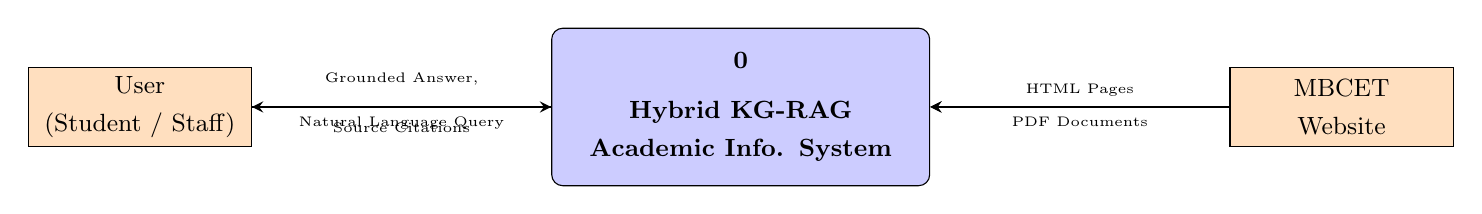
\begin{tikzpicture}[node distance=1.8cm, every node/.style={font=\small}]

  % Central process
  \node (sys) [process, minimum width=4.8cm, minimum height=2cm, text width=4.4cm,
               fill=blue!20, font=\small\bfseries]
               {0\\[4pt]Hybrid KG-RAG\\Academic Info. System};

  % External entities
  \node (user)    [entity, left=3.8cm of sys,  fill=orange!25] {User\\(Student / Staff)};
  \node (website) [entity, right=3.8cm of sys, fill=orange!25] {MBCET\\Website};

  % User arrows
  \draw[arrow] (sys) -- node[above, sloped, yshift=4pt]{\tiny Grounded Answer,}
                         node[below, sloped, yshift=-2pt]{\tiny Source Citations} (user);
  \draw[arrow] (user) -- node[below, sloped]{\tiny Natural Language Query} (sys);

  % Website arrows
  \draw[arrow] (website) -- node[above, sloped]{\tiny HTML Pages} (sys);
  \draw[arrow] (website) -- node[below, sloped]{\tiny PDF Documents} (sys);

\end{tikzpicture}
\caption{DFD Level 0 — Context Diagram}
\label{fig:dfd0}
\end{figure}

The MBCET website provides raw HTML pages (faculty profiles, department information, program details) and PDF documents (syllabi, regulations, examination schedules). The system processes both data streams, builds a searchable knowledge base, and returns grounded answers with source citations to the user in response to natural-language queries.

\section{Data Flow Diagram — Level 1}

The Level~1 DFD decomposes the system into six sub-processes, three data stores, and the same two external entities.

\begin{figure}[h!]
\centering
\resizebox{\textwidth}{!}{%
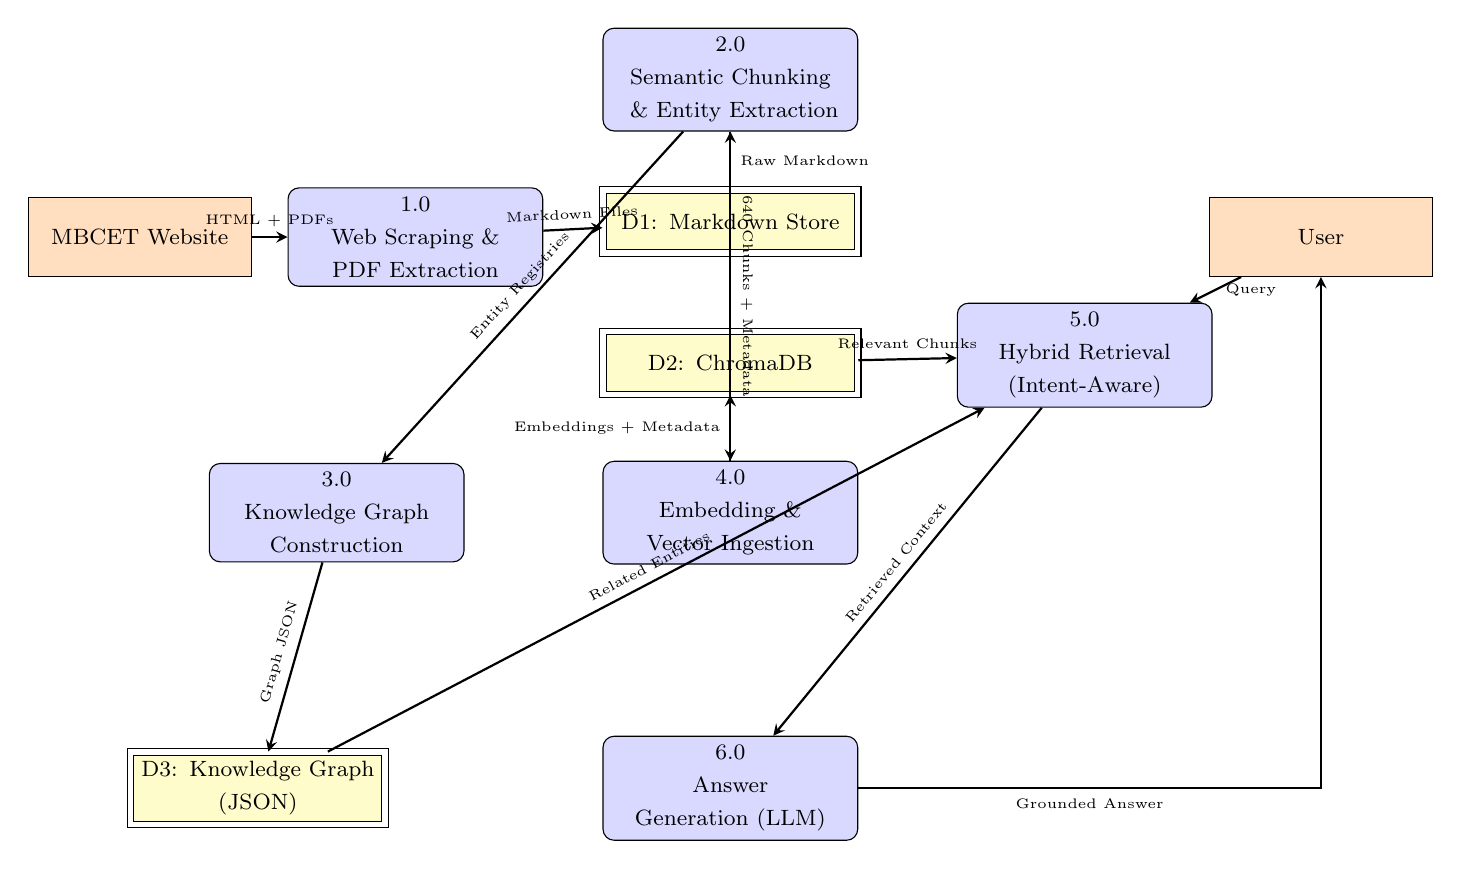
\begin{tikzpicture}[node distance=1.5cm and 2cm, every node/.style={font=\footnotesize}]

  % External entities
  \node (website) [entity, fill=orange!25] at (0, 0)    {MBCET Website};
  \node (user)    [entity, fill=orange!25] at (15, 0)   {User};

  % Processes
  \node (p1) [process, fill=blue!15] at (3.5,    0)   {1.0\\Web Scraping \&\\PDF Extraction};
  \node (p2) [process, fill=blue!15] at (7.5,  2)     {2.0\\Semantic Chunking\\\ \& Entity Extraction};
  \node (p3) [process, fill=blue!15] at (2.5, -3.5)   {3.0\\Knowledge Graph\\Construction};
  \node (p4) [process, fill=blue!15] at (7.5, -3.5)   {4.0\\Embedding \&\\Vector Ingestion};
  \node (p5) [process, fill=blue!15] at (12, -1.5)    {5.0\\Hybrid Retrieval\\(Intent-Aware)};
  \node (p6) [process, fill=blue!15] at (7.5, -7)     {6.0\\Answer\\Generation (LLM)};

  % Data stores
  \node (ds1) [datastore, fill=yellow!20] at (7.5,  0.2)  {D1: Markdown Store};
  \node (ds2) [datastore, fill=yellow!20] at (7.5, -1.6)  {D2: ChromaDB};
  \node (ds3) [datastore, fill=yellow!20] at (1.5, -7)     {D3: Knowledge Graph\\(JSON)};

  % Website -> P1
  \draw[arrow] (website) -- node[above]{\tiny HTML + PDFs} (p1);
  % P1 -> DS1
  \draw[arrow] (p1) -- node[above, sloped]{\tiny Markdown Files} (ds1);
  % DS1 -> P2
  \draw[arrow] (ds1) -- node[right]{\tiny Raw Markdown} (p2);
  % P2 -> P4
  \draw[arrow] (p2) -- node[above, sloped]{\tiny 640 Chunks + Metadata} (p4);
  % P2 -> P3
  \draw[arrow] (p2) -- node[above, sloped]{\tiny Entity Registries} (p3);
  % P3 -> DS3
  \draw[arrow] (p3) -- node[above, sloped]{\tiny Graph JSON} (ds3);
  % P4 -> DS2
  \draw[arrow] (p4) -- node[left]{\tiny Embeddings + Metadata} (ds2);
  % User -> P5
  \draw[arrow] (user) -- node[right]{\tiny Query} (p5);
  % DS2 -> P5
  \draw[arrow] (ds2) -- node[above]{\tiny Relevant Chunks} (p5);
  % DS3 -> P5
  \draw[arrow] (ds3) -- node[above, sloped]{\tiny Related Entities} (p5);
  % P5 -> P6
  \draw[arrow] (p5) -- node[above, sloped]{\tiny Retrieved Context} (p6);
  % P6 -> User (curved)
  \draw[arrow] (p6) -| node[below, near start]{\tiny Grounded Answer} (user);

\end{tikzpicture}
}%
\caption{DFD Level 1 — Expanded System Data Flows}
\label{fig:dfd1}
\end{figure}

Process~1.0 (\textit{Web Scraping \& PDF Extraction}) crawls the MBCET website and converts content to Markdown. Process~2.0 (\textit{Semantic Chunking \& Entity Extraction}) splits Markdown into classified chunks with entity references. Process~3.0 (\textit{Knowledge Graph Construction}) builds the deterministic JSON knowledge graph from entities and chunks. Process~4.0 (\textit{Embedding \& Vector Ingestion}) generates embeddings and stores them in ChromaDB. Process~5.0 (\textit{Hybrid Retrieval}) classifies the user query by intent and retrieves relevant chunks and entities. Process~6.0 (\textit{Answer Generation}) assembles the context and invokes the LLM to produce a grounded response.

\section{System Architecture}

Figure~\ref{fig:sysarch} depicts the layered system architecture.

\begin{figure}[h!]
\centering
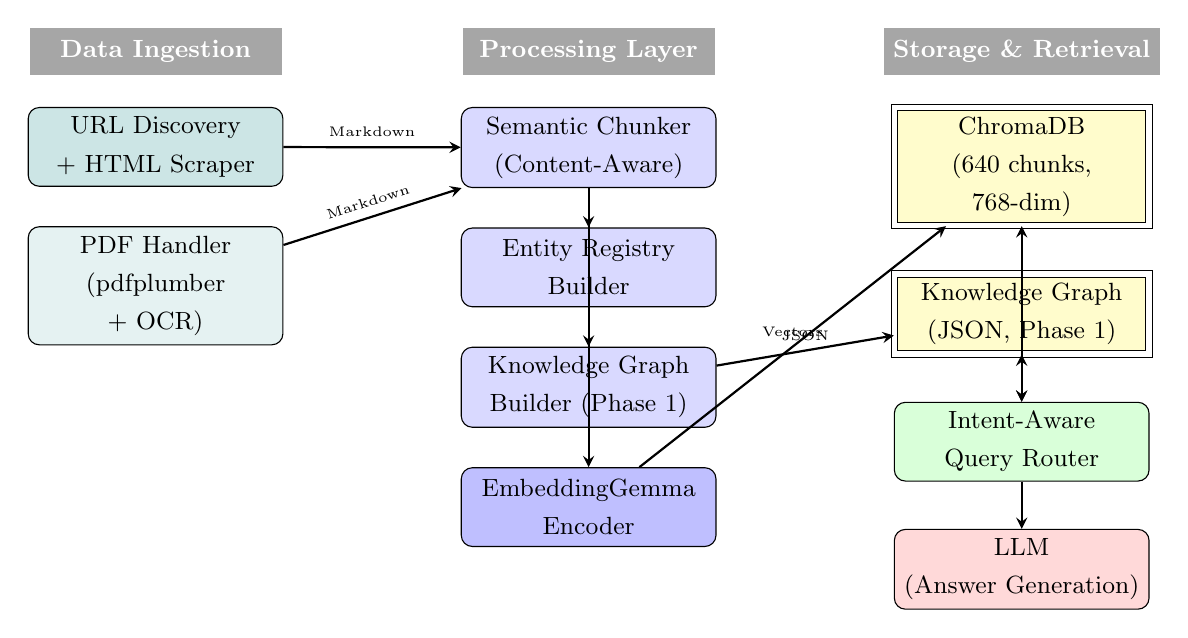
\begin{tikzpicture}[node distance=0.55cm, every node/.style={font=\small}]

  % --- Data Ingestion Layer ---
  \node (d_lbl) [font=\bfseries\small, text=white, fill=gray!70,
                 minimum width=3.2cm, minimum height=0.6cm, align=center]
                 at (0,0) {Data Ingestion};
  \node (scraper) [process, fill=teal!20, below=0.4cm of d_lbl, minimum width=3cm]
                    {URL Discovery\\+ HTML Scraper};
  \node (pdfproc) [process, fill=teal!10, below=0.5cm of scraper, minimum width=3cm]
                    {PDF Handler\\(pdfplumber + OCR)};

  % --- Processing Layer ---
  \node (p_lbl) [font=\bfseries\small, text=white, fill=gray!70,
                 minimum width=3.2cm, minimum height=0.6cm, align=center]
                 at (5.5,0) {Processing Layer};
  \node (chunker)  [process, fill=blue!15, below=0.4cm of p_lbl, minimum width=3cm]
                   {Semantic Chunker\\(Content-Aware)};
  \node (entity)   [process, fill=blue!15, below=0.5cm of chunker, minimum width=3cm]
                   {Entity Registry\\Builder};
  \node (kgbuild)  [process, fill=blue!15, below=0.5cm of entity, minimum width=3cm]
                   {Knowledge Graph\\Builder (Phase 1)};
  \node (embedder) [process, fill=blue!25, below=0.5cm of kgbuild, minimum width=3cm]
                   {EmbeddingGemma\\Encoder};

  % --- Storage Layer ---
  \node (s_lbl) [font=\bfseries\small, text=white, fill=gray!70,
                 minimum width=3.2cm, minimum height=0.6cm, align=center]
                 at (11,0) {Storage \& Retrieval};
  \node (chromadb)  [datastore, fill=yellow!20, below=0.4cm of s_lbl, minimum width=3cm]
                    {ChromaDB\\(640 chunks, 768-dim)};
  \node (kgstore)   [datastore, fill=yellow!20, below=0.6cm of chromadb, minimum width=3cm]
                    {Knowledge Graph\\(JSON, Phase 1)};
  \node (router)    [process, fill=green!15, below=0.6cm of kgstore, minimum width=3cm]
                    {Intent-Aware\\Query Router};
  \node (llm)       [process, fill=red!15, below=0.6cm of router, minimum width=3cm]
                    {LLM\\(Answer Generation)};

  % Arrows
  \draw[arrow] (scraper) -- node[above]{\tiny Markdown} (chunker);
  \draw[arrow] (pdfproc) -- node[above, sloped]{\tiny Markdown} (chunker);
  \draw[arrow] (chunker) -- (entity);
  \draw[arrow] (entity) -- (kgbuild);
  \draw[arrow] (chunker) -- (embedder);
  \draw[arrow] (embedder) -- node[above]{\tiny Vectors} (chromadb);
  \draw[arrow] (kgbuild) -- node[above]{\tiny JSON} (kgstore);
  \draw[darrow] (router) -- (chromadb);
  \draw[darrow] (router) -- (kgstore);
  \draw[arrow] (router) -- (llm);

\end{tikzpicture}
\caption{System Architecture}
\label{fig:sysarch}
\end{figure}

\section{Use Case Diagram}

%TODO: Include use case diagram image if available (e.g., from presentation Images folder)
% \begin{figure}[h!]
%   \centering
%   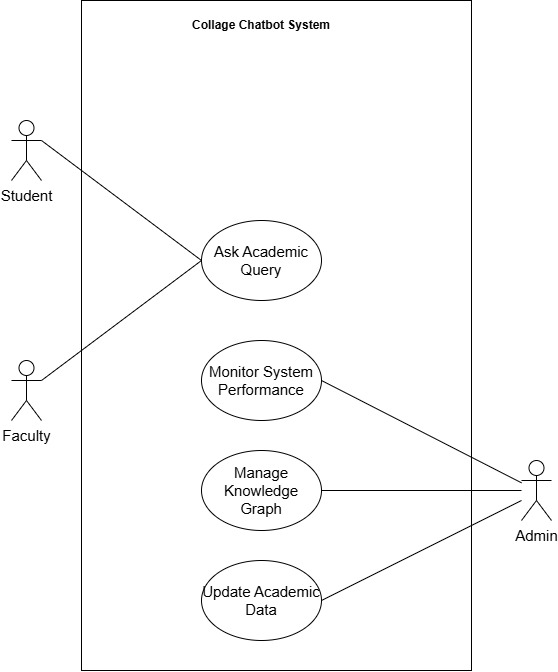
\includegraphics[width=0.5\textwidth]{Images/use_case_noarrow.jpg}
%   \caption{Use Case Diagram}
%   \label{fig:usecase}
% \end{figure}

The primary actors are:
\begin{itemize}
  \item \textbf{Student / End User:} Submits natural-language queries about academic information (courses, faculty, regulations, schedules).
  \item \textbf{Administrator:} Manages the data pipeline (runs scraping, re-indexing, model updates).
\end{itemize}

Key use cases include:
\begin{enumerate}
  \item Query about faculty information (``Who is the HOD of CSE?'')
  \item Query about course details (``How many credits does Computer Networks have?'')
  \item Query about teaching assignments (``Who teaches Artificial Intelligence?'')
  \item Query about regulations (``What is the attendance requirement?'')
  \item Run scraping pipeline (Administrator)
  \item Rebuild knowledge graph (Administrator)
  \item Re-index embeddings (Administrator)
\end{enumerate}

\section{Class Diagram}

%TODO: Include class diagram image if available
% \begin{figure}[h!]
%   \centering
%   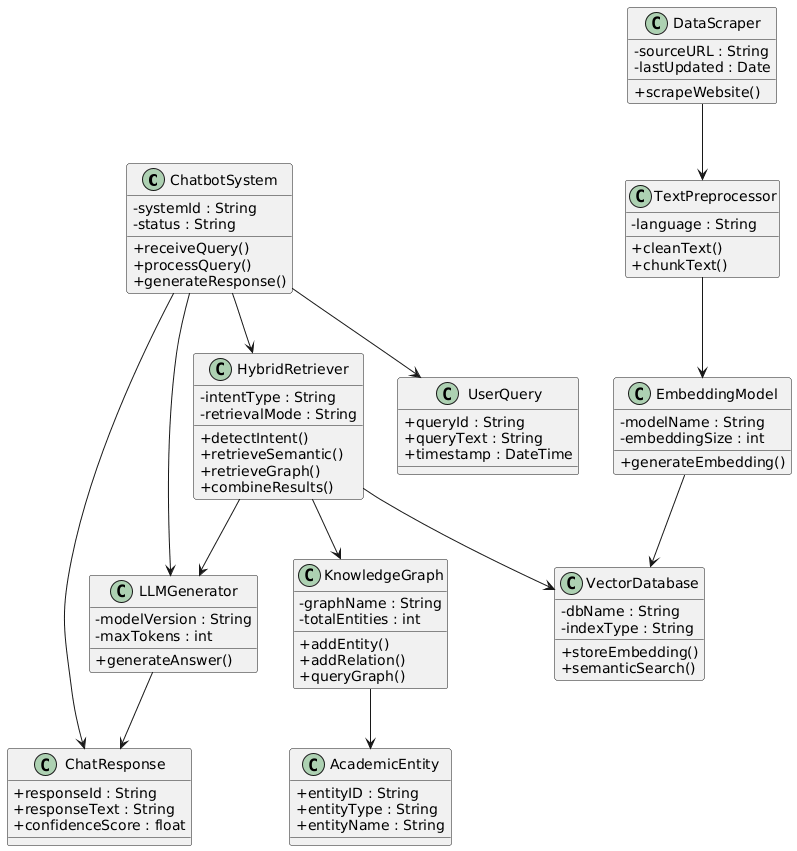
\includegraphics[width=0.55\textwidth]{Images/class_diagram.png}
%   \caption{Class Diagram}
%   \label{fig:classdiag}
% \end{figure}

The core classes in the system are:

\begin{table}[h!]
  \centering
  \caption{Key Classes and Their Responsibilities}
  \label{tab:classes}
  \vspace*{5pt}
  \begin{tabular}{|l|l|p{5.5cm}|}
    \hline
    \textbf{Module} & \textbf{Class/Function} & \textbf{Responsibility} \\ \hline
    \texttt{url\_discovery}     & \texttt{discover\_urls()}        & BFS URL crawling with depth/pattern control \\ \hline
    \texttt{html\_scraper}      & \texttt{HTMLScraper}             & HTML$\rightarrow$Markdown, faculty list extraction \\ \hline
    \texttt{pdf\_handler}       & \texttt{PDFHandler}              & PDF text/table extraction, OCR fallback \\ \hline
    \texttt{semantic\_chunker}  & \texttt{run\_chunking\_pipeline()} & Content-aware splitting, typing, dedup \\ \hline
    \texttt{entity\_registry}   & \texttt{EntityRegistry}          & Entity extraction, ID gen., alias normalisation \\ \hline
    \texttt{content\_classifier}& \texttt{classify\_content()}     & Rule-based content type assignment \\ \hline
    \texttt{builder}            & \texttt{build\_knowledge\_graph()} & Node/edge construction, validation \\ \hline
    \texttt{rag\_ingestion}     & \texttt{run\_ingestion\_pipeline()} & Embedding gen., ChromaDB ingestion \\ \hline
    \texttt{rag\_ingestion}     & \texttt{query\_chromadb()}       & Intent routing, adaptive thresholding \\ \hline
  \end{tabular}
\end{table}

\section{Sequence Diagram}

%TODO: Include sequence diagram image if available
% \begin{figure}[h!]
%   \centering
%   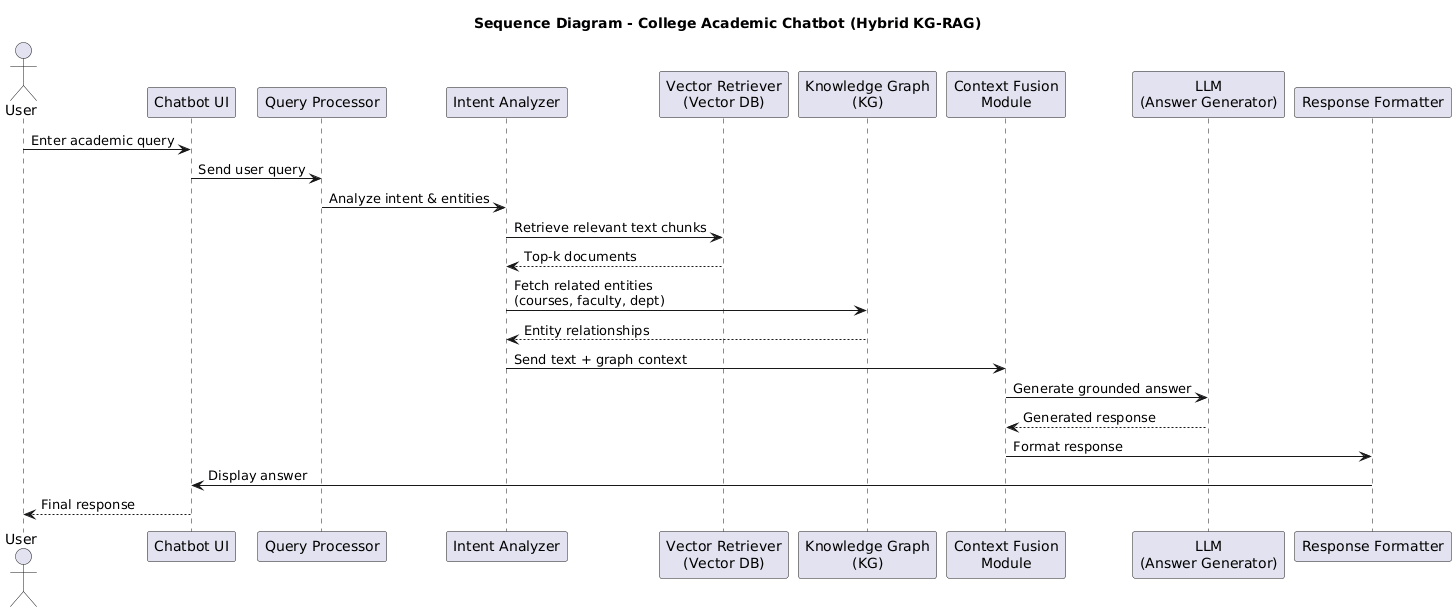
\includegraphics[width=\textwidth]{Images/sequence_diagram.png}
%   \caption{Sequence Diagram — Query Processing Flow}
%   \label{fig:seqdiag}
% \end{figure}

The query processing flow follows these steps:
\begin{enumerate}
  \item User submits a natural-language query via the chatbot interface.
  \item The \texttt{classify\_query\_type()} function analyses the query text against keyword patterns and assigns a query type (teaching, faculty, course, regulation, general).
  \item The query router selects the appropriate retrieval strategy and content-type filter.
  \item The EmbeddingGemma model encodes the query into a 768-dimensional vector.
  \item ChromaDB performs a filtered similarity search, returning the top-$k$ most relevant chunks.
  \item For teaching queries, the knowledge graph is additionally consulted for entity relationships.
  \item Adaptive distance thresholding filters out low-quality matches.
  \item The retrieved context (chunks + graph entities) is assembled and passed to the LLM.
  \item The LLM generates a grounded response and returns it to the user.
\end{enumerate}

\section{Entity-Relationship (ER) Diagram}

\begin{figure}[h!]
\centering
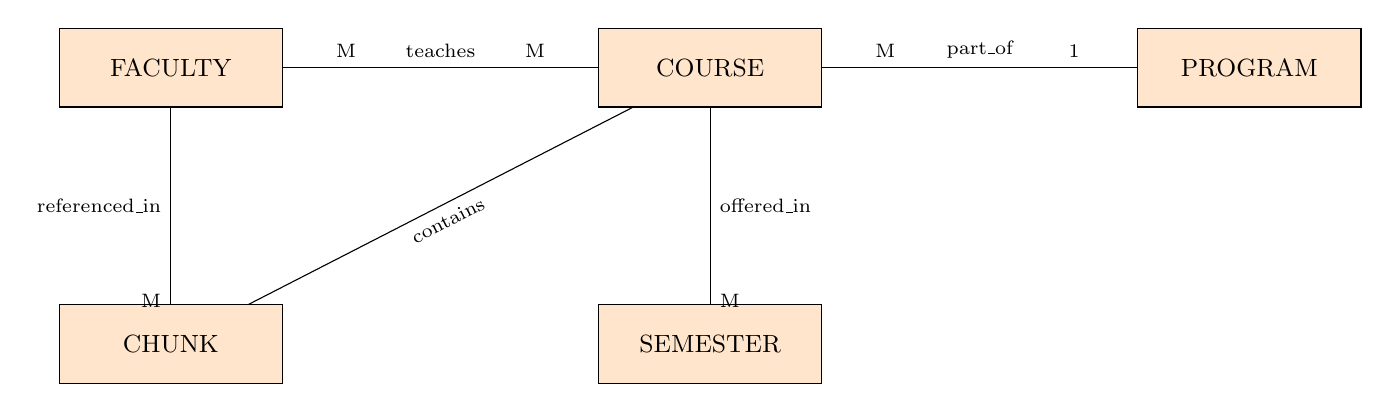
\begin{tikzpicture}[node distance=2.2cm, every node/.style={font=\small}]
  \node (faculty)  [entity, fill=orange!20, minimum width=2.5cm] {FACULTY};
  \node (course)   [entity, fill=orange!20, minimum width=2.5cm, right=4cm of faculty] {COURSE};
  \node (program)  [entity, fill=orange!20, minimum width=2.5cm, right=4cm of course]  {PROGRAM};
  \node (chunk)    [entity, fill=orange!20, minimum width=2.5cm, below=2.5cm of faculty] {CHUNK};
  \node (semester) [entity, fill=orange!20, minimum width=2.5cm, below=2.5cm of course]  {SEMESTER};

  \draw (faculty) -- node[above]{\scriptsize teaches} node[above, xshift=-1.2cm]{\scriptsize M} node[above, xshift=1.2cm]{\scriptsize M} (course);
  \draw (course)  -- node[above]{\scriptsize part\_of} node[above, xshift=-1.2cm]{\scriptsize M} node[above, xshift=1.2cm]{\scriptsize 1} (program);
  \draw (faculty) -- node[left]{\scriptsize referenced\_in} node[left, yshift=-1.2cm]{\scriptsize M} (chunk);
  \draw (course)  -- node[right]{\scriptsize offered\_in} node[right, yshift=-1.2cm]{\scriptsize M} (semester);
  \draw (chunk)   -- node[below, sloped]{\scriptsize contains} (course);
\end{tikzpicture}
\caption{Entity-Relationship Diagram}
\label{fig:er}
\end{figure}

The ER diagram captures the core relationships in the knowledge graph: faculty members teach courses, courses belong to programs, courses are offered in specific semesters, and chunks reference both faculty and course entities.

\section{Pipeline Output Summary}

\begin{table}[h!]
  \centering
  \caption{Pipeline Stage Outputs}
  \label{tab:pipeline_outputs}
  \vspace*{5pt}
  \begin{tabular}{|l|c|l|}
    \hline
    \textbf{Stage} & \textbf{Count} & \textbf{Output Location} \\ \hline
    HTML pages scraped    & 60+  & \texttt{data/markdown/pages/}     \\ \hline
    PDFs processed        & 10   & \texttt{data/markdown/pdfs/}      \\ \hline
    Faculty entities      & 43   & \texttt{data/entities/faculty.json} \\ \hline
    Semantic chunks       & 640  & \texttt{data/chunks/chunks.json}  \\ \hline
    Duplicates detected   & 1    & (skipped during chunking)         \\ \hline
    KG nodes              & ---  & \texttt{data/knowledge\_graph/graph.json} \\ \hline
    KG edges              & ---  & \texttt{data/knowledge\_graph/graph.json} \\ \hline
    ChromaDB vectors      & 640+ & \texttt{chroma\_db/}              \\ \hline
    Unit tests passing    & 50   & \texttt{tests/}                   \\ \hline
  \end{tabular}
\end{table}

\clearpage

%% ============================================================
%%  REFERENCES
%% ============================================================
\bibliographystyle{ieeetr}
\begin{thebibliography}{99}

  \bibitem{kg_rag_springer}
  J.~Linders and J.~M.~Tomczak,
  ``Knowledge graph-extended retrieval augmented generation for question answering,''
  \emph{Applied Intelligence}, vol.~55, no.~17, pp.~1102--1118, 2025.

  \bibitem{rag_edu_elsevier}
  Z.~Li, Z.~Wang, W.~Wang, K.~Hung, H.~Xie, and F.~L.~Wang,
  ``Retrieval-augmented generation for educational application: A systematic survey,''
  \emph{Computers and Education: Artificial Intelligence}, vol.~8, p.~100417, 2025.

  \bibitem{lewis2020}
  P.~Lewis, E.~Perez, A.~Piktus, F.~Petroni, V.~Karpukhin, N.~Goyal,
  H.~K\"{u}ttler, M.~Lewis, W.-T.~Yih, T.~Rockt\"{a}schel, S.~Riedel, and D.~Kiela,
  ``Retrieval-augmented generation for knowledge-intensive NLP tasks,''
  in \emph{Advances in Neural Information Processing Systems (NeurIPS)}, vol.~33,
  pp.~9459--9474, 2020.

  \bibitem{izacard2021}
  G.~Izacard and E.~Grave,
  ``Leveraging passage retrieval with generative models for open domain question answering,''
  in \emph{Proc.\ 16th Conference of the European Chapter of the ACL (EACL)},
  pp.~874--880, 2021.

  \bibitem{hogan2021}
  A.~Hogan, E.~Blomqvist, M.~Cochez, C.~d'Amato, G.~de~Melo, C.~Gutierrez,
  S.~Kirrane, J.~E.~L\'{a}baj N\'{a}ter, R.~Navigli, S.~Neumaier, A.-C.~Ngonga~Ngomo,
  A.~Polleres, S.~M.~Rashid, A.~Rula, L.~Schmelzeisen, J.~Sequeda, S.~Staab,
  and A.~Zimmermann,
  ``Knowledge graphs,''
  \emph{ACM Computing Surveys}, vol.~54, no.~4, pp.~1--37, 2021.

  \bibitem{pan2024}
  S.~Pan, L.~Luo, Y.~Wang, C.~Chen, J.~Wang, and X.~Wu,
  ``Unifying large language models and knowledge graphs: A roadmap,''
  \emph{IEEE Transactions on Knowledge and Data Engineering}, vol.~36, no.~7,
  pp.~3580--3599, 2024.

\end{thebibliography}

\end{document}
